%! TEX root = ../Slides.tex
\chapter{CFD-DEM Coupling}


% Overview Slide
\begin{frame}{Overview of Coupling Methodologies}
    Fluid-particle interactions govern many critical processes. The choice of methodology depends heavily on the required resolution, scale, and available computational resources.
    \vspace{0.5cm}
    
    \textbf{Primary Methods Discussed:}
    \begin{itemize}
        \item Under-Resolved (Unresolved) CFD-DEM
        \item Fully Resolved CFD-DEM
        \item Pore Model (Pore-Scale)
        \item Lattice Boltzmann Method (LBM-DEM)
        \item Smoothed Particle Hydrodynamics (SPH-DEM)
        \item Immersed Boundary Method (IBM-DEM)
        \item Volume of Fluids (VOF-DEM)
    \end{itemize}
\end{frame}

% 1. Under-Resolved CFD-DEM
\begin{frame}{1. Under-Resolved CFD-DEM}
    \textbf{Concept:} Fluid mesh cells are significantly larger than individual particles. Fluid properties are locally averaged, and interactions are based on empirical drag models.
    \vspace{0.3cm}
    
    \begin{columns}[T]
        \begin{column}{0.48\textwidth}
            \begin{block}{Pros}
                \begin{itemize}
                    \item Highly computationally efficient.
                    \item Suitable for large-scale, industrial simulations (millions of particles).
                    \item Robust empirical drag models are well-established.
                \end{itemize}
            \end{block}
        \end{column}
        
        \begin{column}{0.48\textwidth}
            \begin{alertblock}{Cons}
                \begin{itemize}
                    \item Lacks detailed flow resolution around individual particles.
                    \item Heavily reliant on empirical correlations.
                    \item Struggles with highly dense beds or complex particle shapes.
                \end{itemize}
            \end{alertblock}
        \end{column}
    \end{columns}
\end{frame}

% 2. Fully Resolved CFD-DEM
\begin{frame}{2. Fully Resolved CFD-DEM}
    \textbf{Concept:} The CFD mesh is significantly smaller than the particles, capturing the exact flow field and boundary layer around every single particle directly.
    \vspace{0.3cm}
    
    \begin{columns}[T]
        \begin{column}{0.48\textwidth}
            \begin{block}{Pros}
                \begin{itemize}
                    \item Provides fundamental insights into local hydrodynamics.
                    \item No need for empirical drag models.
                    \item Excellent for studying non-spherical and complex particle shapes.
                \end{itemize}
            \end{block}
        \end{column}
        
        \begin{column}{0.48\textwidth}
            \begin{alertblock}{Cons}
                \begin{itemize}
                    \item Extremely computationally expensive.
                    \item Limited to small domains (thousands, not millions of particles).
                    \item Mesh generation and dynamic updating are highly complex.
                \end{itemize}
            \end{alertblock}
        \end{column}
    \end{columns}
\end{frame}
\mode<article>{It should be noted that to reduce the computation cost the particles are often scaled up (see section when written) to reduce the particles number. This requires correct rescaling of all of the forces between the two methods.


}

% 3. Pore Model
\begin{frame}{3. Pore Model (Pore Network)}
    \textbf{Concept:} Represents the void space between particles as a network of interconnected pores and throats, solving for network conductivity rather than full Navier-Stokes equations.
    \vspace{0.3cm}
    
    \begin{columns}[T]
        \begin{column}{0.48\textwidth}
            \begin{block}{Pros}
                \begin{itemize}
                    \item Computationally faster than fully resolved CFD for porous media.
                    \item Excellent for multi-phase flow and capillary effects.
                    \item Directly links macroscopic permeability to microscopic structure.
                \end{itemize}
            \end{block}
        \end{column}
        
        \begin{column}{0.48\textwidth}
            \begin{alertblock}{Cons}
                \begin{itemize}
                    \item Extracting an accurate pore network from dynamic DEM packing is difficult.
                    \item Typically assumes creeping (low Reynolds number) flow.
                    \item Dynamic coupling (constantly moving particles) is challenging.
                \end{itemize}
            \end{alertblock}
        \end{column}
    \end{columns}
\end{frame}

% 4. Lattice Boltzmann Method (LBM-DEM)
\begin{frame}{4. Lattice Boltzmann Method (LBM-DEM)}
    \textbf{Concept:} Tracks the probability distribution of fictitious fluid particles colliding and streaming over a discrete lattice grid, rather than solving macroscopic Navier-Stokes.
    \vspace{0.3cm}
    
    \begin{columns}[T]
        \begin{column}{0.48\textwidth}
            \begin{block}{Pros}
                \begin{itemize}
                    \item Highly parallelizable; highly efficient on modern GPUs.
                    \item Handles complex/moving boundaries naturally without complex meshing.
                    \item Accurate for transient and aeroacoustic phenomena.
                \end{itemize}
            \end{block}
        \end{column}
        
        \begin{column}{0.48\textwidth}
            \begin{alertblock}{Cons}
                \begin{itemize}
                    \item Higher memory requirements than traditional finite volume methods.
                    \item Can suffer from stability issues at high Reynolds numbers.
                    \item Uniform grid can be inefficient for localized high-resolution needs.
                \end{itemize}
            \end{alertblock}
        \end{column}
    \end{columns}
\end{frame}

% 5. SPH-DEM
\begin{frame}{5. Smoothed Particle Hydrodynamics (SPH-DEM)}
    \textbf{Concept:} A fully meshfree, Lagrangian approach where the fluid is discretised into interacting \lq particles\rq . Both fluid (SPH) and solids (DEM) share a particle-based framework.
    \vspace{0.3cm}
    
    \begin{columns}[T]
        \begin{column}{0.48\textwidth}
            \begin{block}{Pros}
                \begin{itemize}
                    \item No mesh generation or grid entanglement issues.
                    \item Suited for highly dynamic flows, large deformations, and free surfaces.
                    \item Natural tracking of fluid-solid interfaces.
                \end{itemize}
            \end{block}
        \end{column}
        
        \begin{column}{0.48\textwidth}
            \begin{alertblock}{Cons}
                \begin{itemize}
                    \item Enforcing rigorous boundary conditions (like no-slip walls) is complex.
                    \item Prone to numerical over-dissipation or artificial viscosity.
                    \item Generally more computationally expensive per fluid volume than Eulerian methods.
                \end{itemize}
            \end{alertblock}
        \end{column}
    \end{columns}
\end{frame}

% 6. Immersed Boundary Method (IBM-DEM)
\begin{frame}{6. Immersed Boundary Method (IBM-DEM)}
    \textbf{Concept:} A fully resolved approach using a fixed, stationary background fluid grid. Solid boundaries are represented by adding mathematical forcing terms to the Navier-Stokes equations, rather than fitting the mesh to the particle.
    \vspace{0.3cm}
    
    \begin{columns}[T]
        \begin{column}{0.48\textwidth}
            \begin{block}{Pros}
                \begin{itemize}
                    \item Completely avoids computationally expensive dynamic remeshing.
                    \item Highly efficient for simulating moving and interacting boundaries.
                    \item Scales well on parallel computing architectures.
                \end{itemize}
            \end{block}
        \end{column}
        
        \begin{column}{0.48\textwidth}
            \begin{alertblock}{Cons}
                \begin{itemize}
                    \item The solid-fluid interface is \lq smeared,\rq\ reducing boundary layer accuracy compared to body-fitted meshes.
                    \item High grid resolution is still required to capture the interface forcing accurately.
                \end{itemize}
            \end{alertblock}
        \end{column}
    \end{columns}
   
\end{frame}

%Parcel method
\begin{frame}{7. Coarse-Grained / Parcel CFD-DEM}
    \textbf{Concept:} Groups multiple physical particles into a single computational \lq parcel\rq\ or macroscopic particle to drastically reduce the number of entities tracked in the DEM solver.
    \vspace{0.3cm}
    
    \begin{columns}[T]
        \begin{column}{0.48\textwidth}
            \begin{block}{Pros}
                \begin{itemize}
                    \item The only viable discrete way to model industrial-scale systems (billions of particles).
                    \item Massive reduction in computational time and memory usage.
                \end{itemize}
            \end{block}
        \end{column}
        
        \begin{column}{0.48\textwidth}
            \begin{alertblock}{Cons}
                \begin{itemize}
                    \item Exact microscopic physics (like specific particle-particle collision dynamics) are lost or averaged.
                    \item Requires careful tuning of scaling factors (e.g., spring stiffness) to maintain bulk behaviour.
                \end{itemize}
            \end{alertblock}
        \end{column}
    \end{columns}
\end{frame}

% 8. VOF-DEM (Three-Phase Coupling)
\begin{frame}{8. Volume of Fluid with DEM (VOF-DEM)}
    \textbf{Concept:} Combines standard CFD-DEM with an interface tracking method (VOF) to model systems with interacting particles and two distinct fluid phases (e.g., air and liquid).
    \vspace{0.3cm}
    
    \begin{columns}[T]
        \begin{column}{0.48\textwidth}
            \begin{block}{Pros}
                \begin{itemize}
                    \item Ideal for wet granulation, capillary bridging, and droplet-particle impacts.
                    \item Captures complex free-surface fluid dynamics around moving solids.
                \end{itemize}
            \end{block}
        \end{column}
        
        \begin{column}{0.48\textwidth}
            \begin{alertblock}{Cons}
                \begin{itemize}
                    \item Extremely computationally demanding (requires very fine mesh for the VOF interface).
                    \item Managing surface tension, contact angles, and dynamic contact lines on moving particles is highly complex.
                \end{itemize}
            \end{alertblock}
        \end{column}
    \end{columns}
\end{frame}

% Active Network Codes
\begin{frame}{Active Codes in the Network}
    \textbf{Current CFD-DEM Software Implementations:}
    \vspace{0.4cm}
    
    \begin{columns}[T]
        % Left Column (5 items: a - e)
        \begin{column}{0.48\textwidth}
            \begin{enumerate}[a)]
                \item {Hybrid}
                \item {LIGGGHTS-PreCICE-OpenFOAM}
                \item {Mercury-PreCICE-OpenFOAM}
                \item {MercurySPH-DEM}
                \item {Moomph}
            \end{enumerate}
        \end{column}
        
        % Right Column (4 items: f - i)
        \begin{column}{0.48\textwidth}
            \begin{enumerate}[a)]
                \setcounter{enumi}{5}
                \item {OpenFOAM with internal DEM}
                \item {PhasicFlowPlus}
                \item {Yade-OpenFOAM}
                \item {Yade-PoreFlow}
            \end{enumerate}
        \end{column}
    \end{columns}
\end{frame}

% Summary Mapping Slide
\begin{frame}{Methodology to Code Mapping}
    \textbf{Overview of capabilities within the network:}
    \vspace{0.3cm}
    
    \begin{table}
        \centering
        % Resizes the table to fit the slide width if necessary
        \resizebox{\textwidth}{!}{%
        \begin{tabular}{l cccccccc}
            \toprule
            \textbf{Code / Software} & \textbf{Unresolved} & \textbf{Resolved} & \textbf{Pore Model} & \textbf{LBM} & \textbf{SPH}  &\textbf{IBM} & \textbf{Parcel} & \textbf{VOF}\\
            \midrule
            Hybrid                      &            &            &            &       \checkmark     &         & &   \\
            LIGGGHTS-PreCICE-OpenFOAM   & \checkmark &            &            &            &       & &     \\
            Mercury-PreCICE-OpenFOAM    & \checkmark & (\checkmark) &            &            &     & &       \\
            MercurySPH-DEM              &            &            &            &            & \checkmark  & &\\
            Moomph                      & \checkmark &            &            &            &            & &\\
            OpenFOAM with internal DEM  & \checkmark &            &            &            &   & &         \\
            PhasicFlowPlus              & \checkmark & \checkmark &            &            &          &&  \\
            Yade-OpenFOAM               & \checkmark & \checkmark &            &            &           && \\
            Yade-PoreFlow               &            &            & \checkmark &            &            &&\\
            \bottomrule
        \end{tabular}%
        }
    \end{table}
    
 \end{frame}
    
 % Fully Resolved: Mathematical Framework
\begin{frame}{Fully Resolved CFD-DEM: Mathematical Framework}
    \textbf{Governing Principles}
    \vspace{0.3cm}
    
    In fully-resolved simulations, the equations of motion for the fluid and the particles are solved completely separately.
    
    \begin{itemize}
        \item The fluid is resolved on a scale significantly smaller than the particles (typically $8\pi$ times smaller than the smallest particle diameter).
        \item The fluid strictly follows the incompressible Navier-Stokes equations (continuity and momentum).
        \item Instead of using empirical drag models, all interaction information is passed exactly at the particle-fluid interface ($\Gamma_{pf}$).
        \item To minimise the number of fluid elements in these very dilute systems, mesh-adaptivity can be applied.
    \end{itemize}
\end{frame}

% Fully Resolved: Governing Equations
\begin{frame}{Fully Resolved CFD-DEM: Governing Equations}
    \textbf{Incompressible Navier-Stokes}
    \vspace{0.3cm}
    
    The fluid domain is strictly governed by the conservation of mass (continuity) and momentum.
    
    \vspace{0.2cm}
    \textbf{Continuity Equation:}
    $$ \nabla \cdot \vec{u}_{f} = 0 $$
    
    \vspace{0.2cm}
    \textbf{Momentum Equation:}
    $$ \rho_{f} \left( \frac{\partial \vec{u}_{f}}{\partial t} + \vec{u}_{f} \cdot \nabla \vec{u}_{f} \right) = -\nabla p + \mu \nabla^2 \vec{u}_{f} + \rho_{f} \vec{g} $$
    
    \vspace{0.3cm}
    \small{\textit{Where $\vec{u}_{f}$ is fluid velocity, $\rho_{f}$ is fluid density, $p$ is pressure, $\mu$ is dynamic viscosity, and $\vec{g}$ is gravitational acceleration.}}
\end{frame}

% Fully Resolved: Interfacial Coupling
\begin{frame}{Fully Resolved CFD-DEM: Interfacial Coupling}
    \textbf{Connectivity Conditions at the Boundary}
    \vspace{0.3cm}
    
    The coupling relies on two primary boundary conditions at the particle-fluid interface ($\Gamma_{pf}$), which prescribe velocities and provide the particle with all fluid forces acting on its surface.
    
    \vspace{0.3cm}
    \textbf{1. Kinematic Boundary Condition (No-Slip):}
    $$ \vec{u}_{f} = \vec{u}_{\Gamma_{pf}} \quad \text{on} \quad \Gamma_{pf} $$
    \vspace{0.1cm}
    
    \textbf{2. Dynamic Boundary Condition (Stress Matching):}
    $$ \sigma_{f} \cdot \vec{n} = t_{\Gamma_{pf}} \quad \text{on} \quad \Gamma_{pf} $$
    
    \vspace{0.3cm}
    \small{\textit{Where $\vec{u}_{f}$ is the fluid velocity, $\sigma_{f}$ is the fluid stress tensor, $\vec{n}$ is the normal vector, and $t_{\Gamma_{pf}}$ represents the interface traction}}
\end{frame}

% Fully Resolved: Force Computation
\begin{frame}{Fully Resolved CFD-DEM: Force Computation}
    \textbf{Integrating the Fluid Stress Tensor}
    \vspace{0.3cm}
    
    Forces like buoyancy, virtual mass, and drag do not need to be modelled empirically; they are implicitly captured by integrating the fluid stress tensor ($\sigma_{f}$) over the particle's surface. 
    
    The stress tensor consists of two primary components:
    \begin{itemize}
        \item \textbf{Hydrostatic Pressure:} Because the direction of this force passes directly through the particle's centre-of-mass, it primarily dictates the translational movement of the particle.
        \item \textbf{Deviatoric Stress:} This component determines the particle's rotation. The resulting rotational velocity is calculated after integrating this stress over the entire particle surface.
    \end{itemize}
\end{frame}

% Fully Resolved: Stress Tensor & Torque
\begin{frame}{Fully Resolved CFD-DEM: Stress Tensor \& Torque}
    \textbf{Mathematical Formulation of Interfacial Forces}
    \vspace{0.3cm}
    
    The fluid stress tensor $\sigma_{f}$ explicitly defines both the pressure and viscous shear forces acting on the particle surface.
    
    \vspace{0.2cm}
    \textbf{Fluid Stress Tensor:}
    $$ \sigma_{f} = -p \mathbf{I} + \mu \left( \nabla \vec{u}_{f} + (\nabla \vec{u}_{f})^T \right) $$
    
    \vspace{0.2cm}
    \textbf{Hydrodynamic Torque Calculation:}
    $$ \vec{T}_{f} = \oint_{\Gamma_{pf}} (\vec{r} - \vec{r}_{c}) \times (\sigma_{f} \cdot \vec{n}) \, dA $$
    
    \vspace{0.3cm}
    \small{\textit{Where $\mathbf{I}$ is the identity tensor, $\vec{r}_{c}$ is the particle center of mass, and $\vec{n}$ is the outward surface normal.}}
\end{frame}

%% Fully Resolved: Handling Moving Particles
%
%
%\begin{frame}{Fully Resolved CFD-DEM: Flow Field vs. Mesh Dynamics}
%    \begin{figure}
%        \begin{minipage}{0.48\textwidth}
%            \centering
%            \textbf{Pressure/Velocity Field} \\
%            \vspace{0.1cm}
%            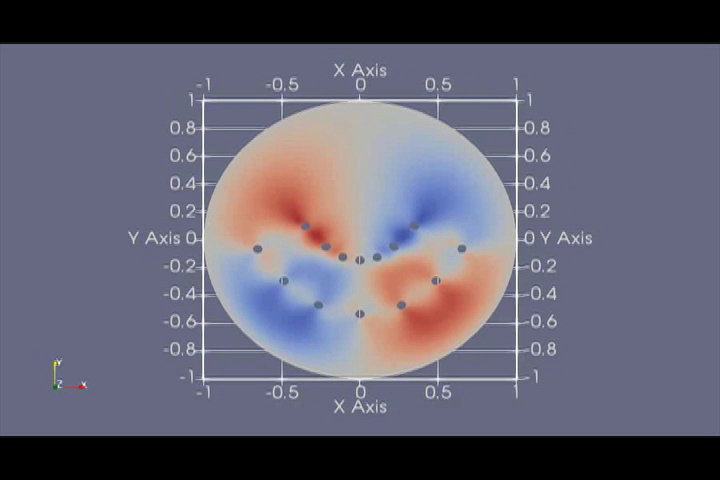
\includegraphics[width=\textwidth]{Images/field_contour.png}
%        \end{minipage}\hfill
%        \begin{minipage}{0.48\textwidth}
%            \centering
%            \textbf{Adaptive Body-Fitted Mesh} \\
%            \vspace{0.1cm}
%            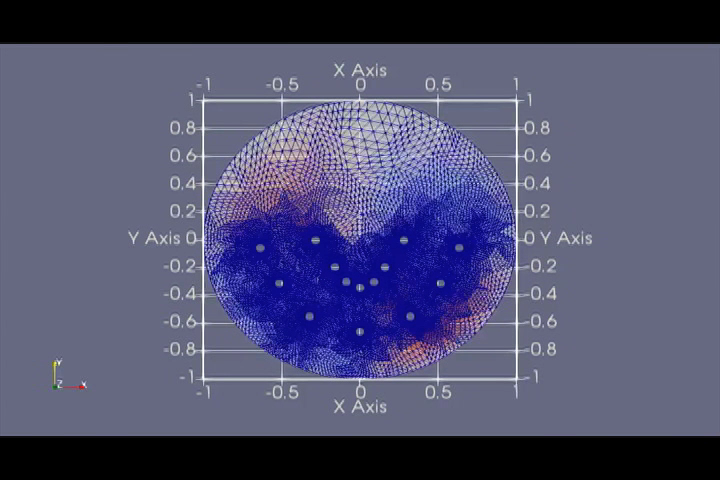
\includegraphics[width=\textwidth]{Images/deformed_mesh.png}
%        \end{minipage}
%    \end{figure}
%    
%    \textbf{Key Observations from Simulation:}
%    \begin{itemize}
%        \item \textbf{Interfacial Coupling:} Fluid stress tensor is integrated directly over the particle surface boundary without empirical drag correlations.
%        \item \textbf{Dynamic Mesh Adaptation:} Mesh nodes deform continuously as particles descend, with local remeshing triggered in narrow inter-particle gaps.
%    \end{itemize}
%\end{frame}

% Fully Resolved: Adaptive Remeshing
\begin{frame}{Fully Resolved CFD-DEM: Adaptive Remeshing}
    
    \begin{figure}
        \begin{minipage}{0.32\textwidth}
            \centering
            \textbf{1. Flow Field} \\
            \vspace{0.1cm}
            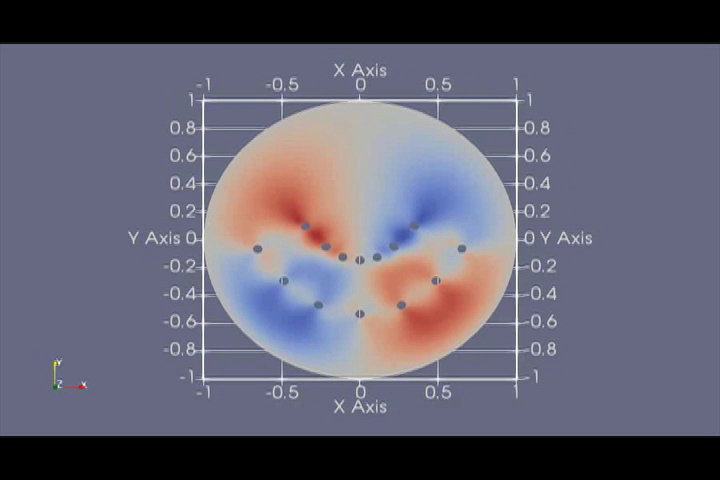
\includegraphics[width=\textwidth]{Images/field_contour.png}
        \end{minipage}\hfill
        \begin{minipage}{0.32\textwidth}
            \centering
            \textbf{2. Initial Mesh} \\
            \vspace{0.1cm}
            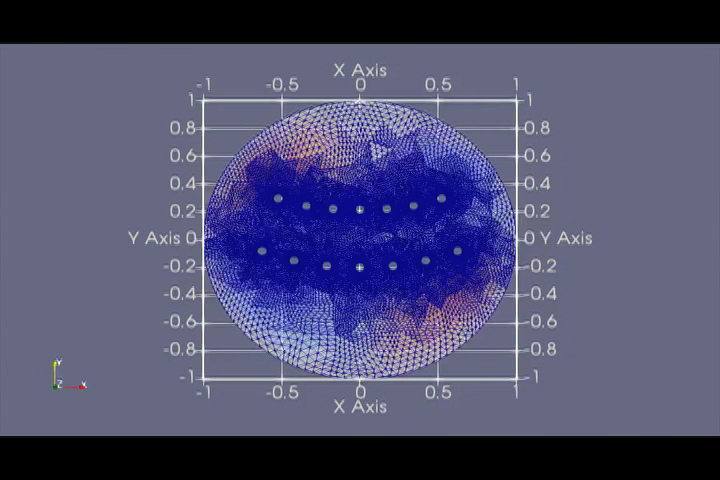
\includegraphics[width=\textwidth]{Images/initial_mesh.png}
        \end{minipage}\hfill
        \begin{minipage}{0.32\textwidth}
            \centering
            \textbf{3. Adapted Mesh} \\
            \vspace{0.1cm}
            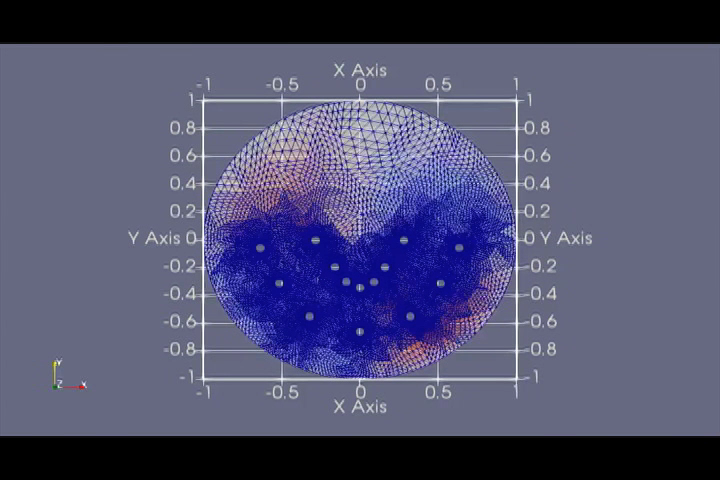
\includegraphics[width=\textwidth]{Images/deformed_mesh.png}
        \end{minipage}
    \end{figure}
    
    \vspace{0.3cm}
    \textbf{Chronological Breakdown:}
    \begin{itemize}
        \item \textbf{Stage 1:} The solver calculates the high-resolution pressure and velocity fields around the particles.
        \item \textbf{Stage 2:} The body-fitted mesh explicitly conforms to the solid particle perimeters.
        \item \textbf{Stage 3 (Adaptive Refinement):} At every time step, the solver evaluates spatial errors and generates a new, refined mesh topology to meet strict error tolerances, particularly in the narrowing gaps.
    \end{itemize}
\end{frame}

\begin{frame}{Acknowledgments: Fully Resolved Implementation}
    \textbf{oomph-lib Framework}
    \vspace{0.3cm}
    
    The fully resolved fluid-particle coupling examples and adaptive remeshing demonstrations shown in this section are built using \textbf{oomph-lib}.
    
    \begin{itemize}
        \item \textbf{Developer:} The core implementation and underlying adaptive meshing routines were developed by Andrew Hazel.
        \item \textbf{Framework:} oomph-lib is an object-oriented, open-source finite-element library explicitly designed for complex multi-physics and fluid-structure interaction problems. %
        
      
    \end{itemize}
\end{frame}

\begin{frame}{Fully Resolved CFD-DEM: Handling Moving Particles}
    \textbf{Why ALE is More Than Just Remeshing}
    \vspace{0.3cm}
    
    Because the mesh is physically fitted to the particle surfaces, the fluid grid must continuously adapt. Doing this efficiently requires moving beyond basic remeshing.
    
    \begin{itemize}
        \item \textbf{The Problem with Simple Remeshing:} Generating a brand-new mesh at every single time step is computationally crushing and introduces severe interpolation errors (numerical diffusion) into the flow field.
        \item \textbf{The ALE Solution (The \lq Rubber Band\rq\ ):} Arbitrary Lagrangian-Eulerian (ALE) methods stretch the existing grid instead. Boundary nodes move exactly with the particle, while internal nodes deform smoothly to absorb the motion.
        \item \textbf{Convective Flux Correction:} Crucially, ALE mathematically modifies the Navier-Stokes equations to subtract the mesh's own velocity, ensuring fluid fluxes remain perfectly accurate across a moving grid.
        \item \textbf{Topological Remeshing (The Fallback):} Only when elements become critically skewed (the rubber band is about to snap) does the solver finally halt, generate a fresh grid, and project the fields.
    \end{itemize}
\end{frame}





% Fully Resolved: Particle Contact
\begin{frame}{Fully Resolved CFD-DEM: Particle Contact}
    \textbf{The Lubrication Singularity \& The Roughness Layer}
    \vspace{0.3cm}
    
    Handling physical particle-particle (and particle-wall) contact is one of the most significant numerical challenges in fully resolved methods.
    
    \vspace{0.2cm}
    \begin{columns}[T]
        \begin{column}{0.48\textwidth}
            \begin{block}{The Problem: Lubrication Singularity}
                \begin{itemize}
                    \item As two smooth spheres approach, the fluid pressure \only<article>{required to squeeze the fluid out of the gap} approaches infinity.
                    \item In a \only<article>{pure} continuum fluid model, the spheres would never \only<article>{actually} touch.
                    \item Furthermore, \only<article>{allowing rigid particles to come into contact} can lead to infinite mesh refinement \only<article>{and crash the CFD solver}.
                \end{itemize}
            \end{block}
        \end{column}
        
        \begin{column}{0.48\textwidth}
            \begin{block}{The Solution: Roughness Layer}
                \begin{itemize}
                    \item A microscopic roughness layer\only<article>{ (or sub-grid lubrication cut-off)} is defined.
                    \item \article{When the gap drops }below this threshold, the CFD lubrication forces are capped.
                    \item The DEM soft-sphere model then takes over\only<article>{, allowing controlled particle overlap to compute mechanical contact forces like friction and elastic repulsion}.
                \end{itemize}
            \end{block}
        \end{column}
    \end{columns}
\end{frame}

\section{Multiresolution}
\only<article>{
Traditional fluid-particle coupling methodologies strictly operate in either fully-resolved or under-resolved regimes, which severely limits their efficiency when simulating suspensions with arbitrarily large particle size distributions. To overcome this limitation, you can couple DEM to FEM in my multi-resolution framework.  This adaptive approach dynamically transitions between fully-resolved fluid boundaries, semi-resolved continuous voidage fields generated via spatial coarse-graining, and under-resolved macroscopic fluid interactions based on the Anderson and Jackson formulation. A comprehensive breakdown of this multi-resolved architecture, its underlying implementation, and the specific coupling mechanics is detailed in \cite{weinhart2020fast}. 
}
\begin{frame}{Particle-Fluid Coupling: Scale Separation}
    
    \begin{figure}
        \begin{minipage}{0.48\textwidth}
            \centering
            \textbf{Fully-Resolved} \\
            \vspace{0.1cm}
            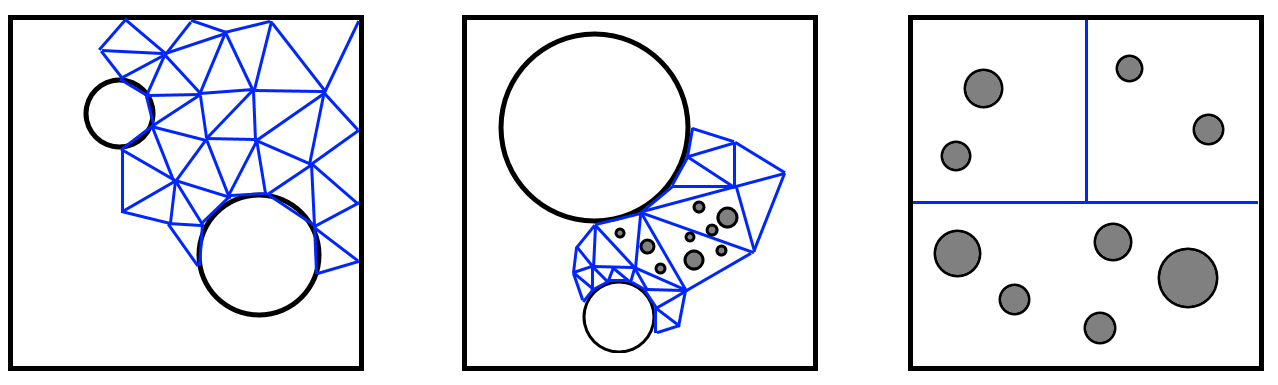
\includegraphics[height=0.45\textheight,clip,trim=0 0 650 0]{Images/resolvedMethods.png}
        \end{minipage}\hfill
        \begin{minipage}{0.48\textwidth}
            \centering
            \textbf{Under-Resolved} \\
            \vspace{0.1cm}
            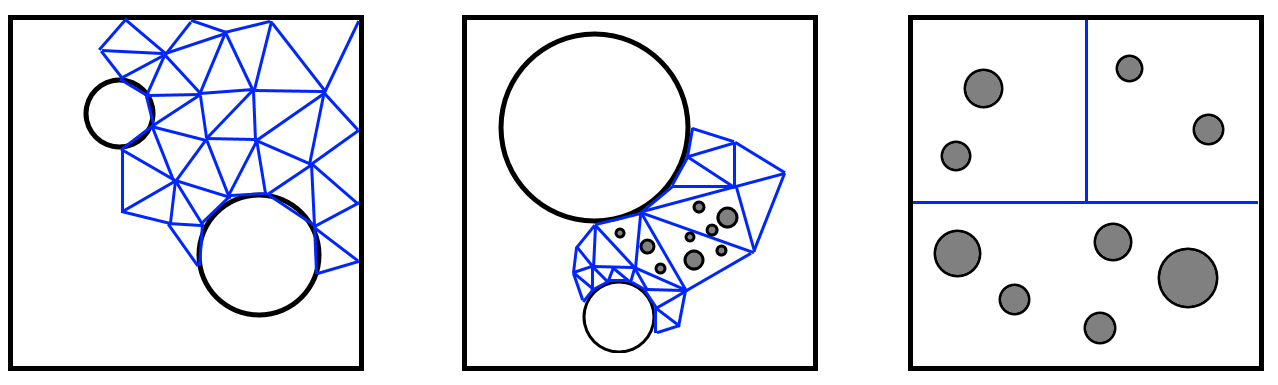
\includegraphics[height=0.45\textheight,clip,trim=650 0 0 0]{Images/resolvedMethods.png}
        \end{minipage}
    \end{figure}
    
    \vspace{0.2cm}
    \textbf{Key Characteristics:}
    \begin{itemize}
        \item \textbf{Fully:} Highly resolved fluid field, but computationally slow. No empirical models needed. Mesh size $h < \frac{1}{8\pi}d_{\text{min}}$.
        \item \textbf{Under:} Low fluid resolution, but fast. Heavily reliant on closure relations (drag models). Mesh size $h > 3d_{\text{max}}$.
    \end{itemize}
    
    \alert{\textbf{Challenge:} Neither method works efficiently for highly polydisperse particle size distributions.} %[cite: 3]
\end{frame}

% Slide 2: The Solution
\begin{frame}{Particle-Fluid Coupling: The Multi-Resolved Approach}
    
    \begin{figure}
        \begin{minipage}{0.32\textwidth}
            \centering \textbf{Fully}
        \end{minipage}\hfill
        \begin{minipage}{0.32\textwidth}
            \centering \textbf{Multi-Resolved}
        \end{minipage}\hfill
        \begin{minipage}{0.32\textwidth}
            \centering \textbf{Under}
        \end{minipage}
        
        \vspace{0.1cm}
        \centering
        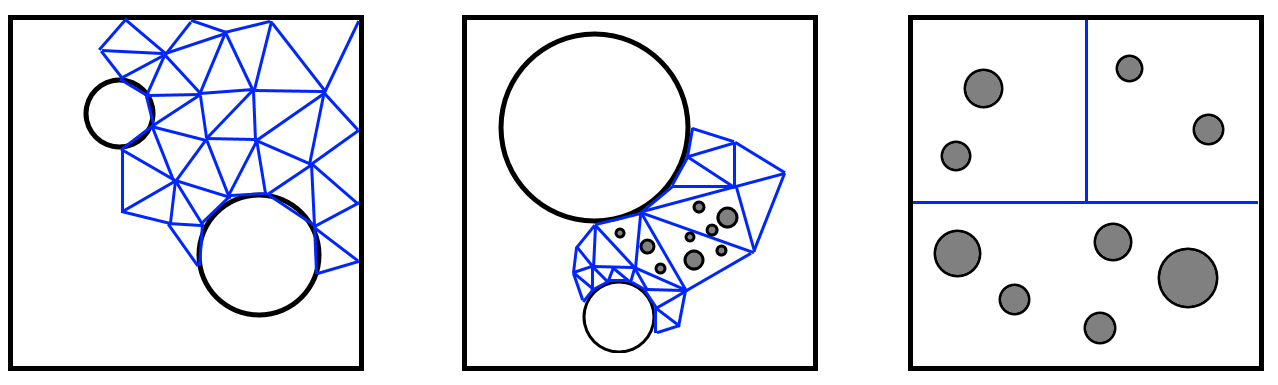
\includegraphics[height=0.35\textheight]{Images/resolvedMethods.png}
    \end{figure}
    
    \vspace{0.2cm}
    \textbf{Key Characteristics:}
    \begin{itemize}
        \item \textbf{Fully:} Highly resolved fluid field, but computationally slow. Mesh size $h < \frac{1}{8\pi}d_{\text{min}}$. %[cite: 3]
        \item \textbf{Under:} Low fluid resolution, but fast. Mesh size $h > 3d_{\text{max}}$.
        \item \alert{\textbf{Multi:}} Bridges the gap by applying fully- and under-resolved simultaneously. It explicitly handles large size ratios and speeds up computation time for complex, realistic processes. %[cite: 3]
    \end{itemize}
\end{frame}

